\section{Software architecture}
\label{sec:C5:software}
In this section, we will present the software architecture of the \textit{Sorotoki} toolkit. The toolkit consists of seven Object-Oriented classes, each designed to address a specific sub-problem within the field of soft robotics. We will introduce each class in the following sequence:

\begin{sidewaysfigure*}
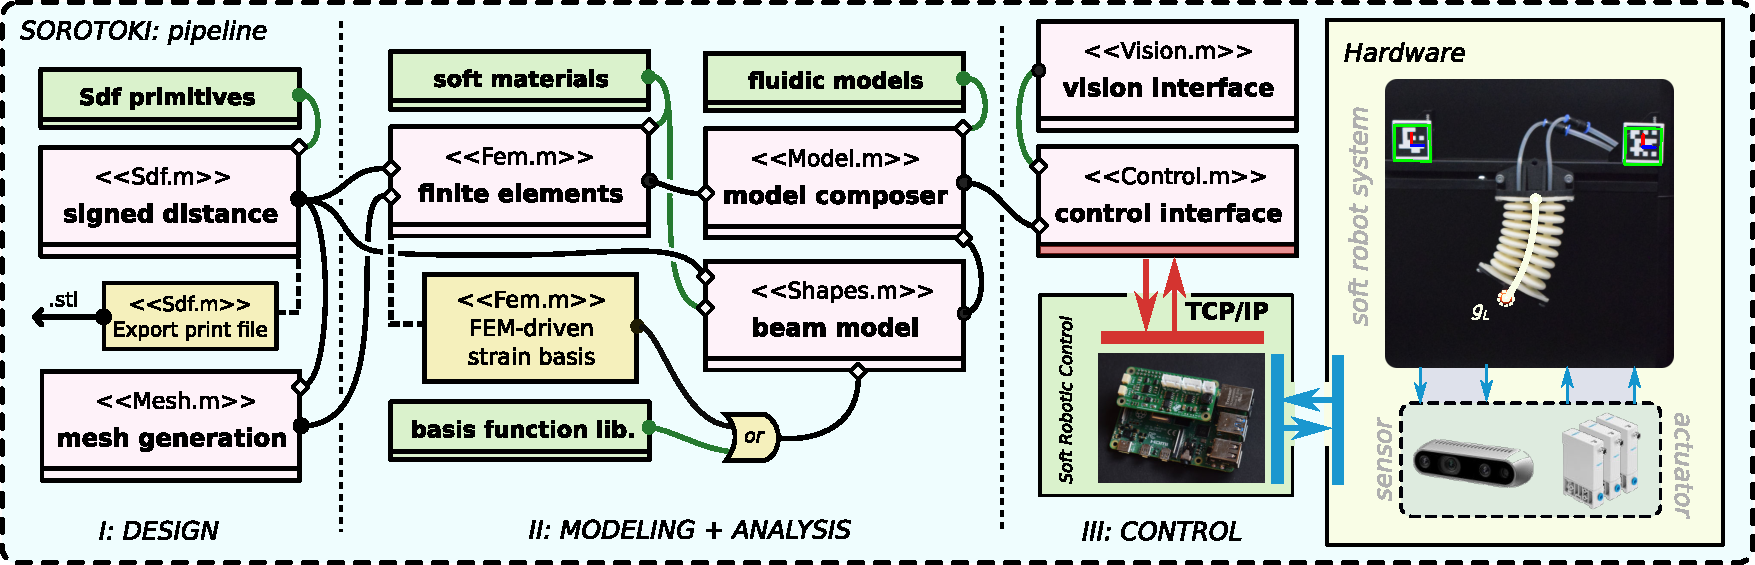
\includegraphics[width=0.955\textwidth]{./pdf/thesis-figure-6-2.pdf}    
\centering
\caption{\small The Sorotoki software toolkit is structured according to a problem-solution pipeline, consisting of seven Object-Oriented classes that address common subproblems in the field of soft robotics research. These classes are: \class{Sdf}, \class{Mesh}, \class{Fem}, \class{Shapes}, \class{Model}, \class{Control}, and \class{Vision}. The software architecture flowchart employs the symbol $(\bullet)$ to represent class outputs and the symbol $(\diamond)$ to denote inputs. It is important to note the interplay between these classes. \label{fig:C5:softwareArchitecture}}
\end{sidewaysfigure*}
%
\begin{itemize}
    \setlength\itemsep{0.0em}
    \item In Section \ref{sec:C5:sdf} we will discuss the class \code{Sdf}: a Signed Distance Function (SDF) class that are used to build spatial geometries --  \emph{"Implicit CAD"};
    \item In Section \ref{sec:C5:mesh} we will discuss \code{Mesh} responsible for mesh generation;
    \item In Section \ref{sec:C5:fem} we discuss the class \code{Fem}: a Finite Element Model (FEM) solver required for high-detail soft robot simulations;
    \item In Section \ref{sec:C5:shapes}, we detail the class \code{Shapes} responsible for soft beam models required for fast soft robot simulations;
    \item In Section \ref{sec:C5:model} we explain \code{Model} -- a model composer to interconnect various dynamic model, and the control synthesis;
    \item Following, in Section \ref{sec:C5:control}, we highlight \code{Control} that serves as a control interface for fluidic platform communicating to \textit{Matlab} via TCP/IP;
    \item Finally, Section \ref{sec:C5:vision} will explain \code{Vision} -- a Vision-based tool for state estimation of soft robots through optical markers.
\end{itemize}
%
To assist the reader, we have included a software architectural flowchart in Figure \ref{fig:C5:softwareArchitecture} that illustrates each class. The flowchart demonstrates how the classes can be interconnected to increase system complexity while maintaining the structured and separable nature of the subproblems. To further clarify their individual functionality, we will provide illustrative examples and corresponding MATLAB executable scripts. The topics covered include design, modeling and analysis, model reduction, and control and vision-based sensing, presented in this chronological order.